    \documentclass{article}

\newif\ifanswers
\answerstrue % comment out to hide answers
\usepackage{bbm}

\usepackage[compact]{titlesec}
\usepackage{fancyhdr} % Required for custom headers
\usepackage{lastpage} % Required to determine the last page for the footer
\usepackage{extramarks} % Required for headers and footers
\usepackage[usenames,dvipsnames]{color} % Required for custom colors
\usepackage{graphicx} % Required to insert images
\usepackage{listings} % Required for insertion of code
\usepackage{courier} % Required for the courier font
\usepackage{lipsum} % Used for inserting dummy 'Lorem ipsum' text into the template
\usepackage{enumerate}
\usepackage{enumitem}
\usepackage{subfigure}
\usepackage{booktabs}
\usepackage{amsmath, amsthm, amssymb}
\allowdisplaybreaks
\usepackage{caption}
\usepackage{hyperref}
\captionsetup[table]{skip=4pt}
\usepackage{framed}
\usepackage{bm}
\usepackage[cache=false]{minted}

\usepackage{tikz}
\usetikzlibrary{positioning,patterns,fit}

% Margins
\topmargin=-0.45in
\evensidemargin=0in
\oddsidemargin=0in
\textwidth=6.5in
\textheight=9.0in
\headsep=0.25in

\linespread{1.1} % Line spacing

% Set up the header and footer
\pagestyle{fancy}
\rhead{\hmwkAuthorName} % Top left header
\lhead{\hmwkClass: \hmwkTitle} % Top center head
\lfoot{\lastxmark} % Bottom left footer
\cfoot{} % Bottom center footer
\rfoot{Page\ \thepage\ of\ \protect\pageref{LastPage}} % Bottom right footer
\renewcommand\headrulewidth{0.4pt} % Size of the header rule
\renewcommand\footrulewidth{0.4pt} % Size of the footer rule

\setlength\parindent{0pt} % Removes all indentation from paragraphs

\newenvironment{answer}{
    % Uncomment this if using the template to write out your solutions.
    {\bf Answer:} \sf \begingroup\color{red}
}{\endgroup}%
%----------------------------------------------------------------------------------------
%	CODE INCLUSION CONFIGURATION
%----------------------------------------------------------------------------------------

\definecolor{MyDarkGreen}{rgb}{0.0,0.4,0.0} % This is the color used for comments
\definecolor{shadecolor}{gray}{0.9}

\lstloadlanguages{Python} % Load Perl syntax for listings, for a list of other languages supported see: ftp://ftp.tex.ac.uk/tex-archive/macros/latex/contrib/listings/listings.pdf
\lstset{language=Python, % Use Perl in this example
        frame=single, % Single frame around code
        basicstyle=\footnotesize\ttfamily, % Use small true type font
        keywordstyle=[1]\color{Blue}\bf, % Perl functions bold and blue
        keywordstyle=[2]\color{Purple}, % Perl function arguments purple
        keywordstyle=[3]\color{Blue}\underbar, % Custom functions underlined and blue
        identifierstyle=, % Nothing special about identifiers
        commentstyle=\usefont{T1}{pcr}{m}{sl}\color{MyDarkGreen}\small, % Comments small dark green courier font
        stringstyle=\color{Purple}, % Strings are purple
        showstringspaces=false, % Don't put marks in string spaces
        tabsize=5, % 5 spaces per tab
        %
        % Put standard Perl functions not included in the default language here
        morekeywords={rand},
        %
        % Put Perl function parameters here
        morekeywords=[2]{on, off, interp},
        %
        % Put user defined functions here
        morekeywords=[3]{test},
       	%
        morecomment=[l][\color{Blue}]{...}, % Line continuation (...) like blue comment
        numbers=left, % Line numbers on left
        firstnumber=1, % Line numbers start with line 1
        numberstyle=\tiny\color{Blue}, % Line numbers are blue and small
        stepnumber=5 % Line numbers go in steps of 5
}

% Creates a new command to include a perl script, the first parameter is the filename of the script (without .pl), the second parameter is the caption
\newcommand{\perlscript}[2]{
\begin{itemize}
\item[]\lstinputlisting[caption=#2,label=#1]{#1.pl}
\end{itemize}
}

%----------------------------------------------------------------------------------------
%	NAME AND CLASS SECTION
%----------------------------------------------------------------------------------------

\newcommand{\hmwkTitle}{word2vec (48 Points)} % Assignment title
\newcommand{\hmwkClass}{CS\ 224n Assignment \#2} % Course/class
\newcommand{\hmwkAuthorName}{Shrikant Malviya} % Your name

\newcommand{\ifans}[1]{\ifanswers \color{red} \vspace{5mm} \textbf{Solution: } #1 \color{black} \vspace{5mm} \fi}

% Chris' notes
\definecolor{CMpurple}{rgb}{0.6,0.18,0.64}
\newcommand\cm[1]{\textcolor{CMpurple}{\small\textsf{\bfseries CM\@: #1}}}
\newcommand\cmm[1]{\marginpar{\small\raggedright\textcolor{CMpurple}{\textsf{\bfseries CM\@: #1}}}}

%----------------------------------------------------------------------------------------
%	TITLE PAGE
%----------------------------------------------------------------------------------------
\title{
\vspace{-1in}
\textmd{\textbf{\hmwkClass:\ \hmwkTitle} \\ \hmwkAuthorName}\\
}
\author{}
%\date{\textit{\small Updated \today\ at \currenttime}} % Insert date here if you want it to appear below your name
\date{}

\setcounter{section}{0} % one-indexing
\begin{document}

\maketitle
\vspace{-.7in}

\begin{center}
    \large{\textbf{Due on} Tuesday Jan. 18, 2022 by \textbf{3:15pm (before class)}}
\end{center}

\section{Written: Understanding word2vec (30 points)}
Recall that the key insight behind {\tt word2vec} is that \textit{`a word is known by the company it keeps'}. Concretely, consider a `center' word $c$ surrounded before and after by a context of a certain length. We term words in this contextual window `outside words' ($O$). For example, in Figure~\ref{fig:word2vec}, the context window length is 2, the center word $c$ is `banking', and the outside words are `turning', `into', `crises', and `as':

\begin{figure}[h]
    \centering
    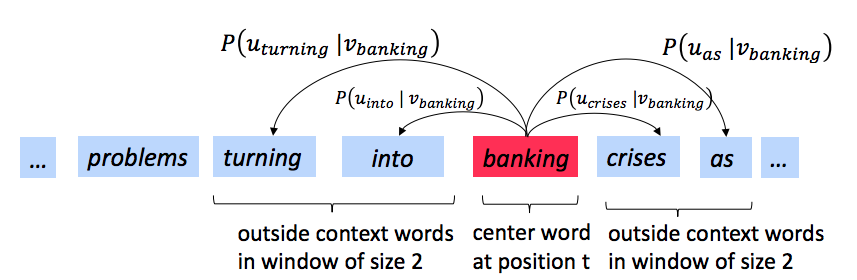
\includegraphics[width=0.6\textwidth]{word2vec.png}
    \caption{The word2vec skip-gram prediction model with window size 2}
    \label{fig:word2vec}
\end{figure}

Skip-gram {\tt word2vec} aims to learn the probability distribution $P(O|C)$. 
Specifically, given a specific word $o$ and a specific word $c$, we want to predict $P(O=o|C=c)$: the probability that word $o$ is an `outside' word for $c$ (i.e., that it falls within the contextual window of $c$).
We model this probability by taking the softmax function over a series of vector dot-products: % I added the word "softmax" here because I bet a lot of students will have forgotten what softmax is and why the loss fn is called naive softmax. but if this is too wordy we can just take it out

\begin{equation}
 P(O=o \mid C=c) = \frac{\exp(\bm u_{o}^\top \bm v_c)}{\sum_{w \in \text{Vocab}} \exp(\bm u_{w}^\top \bm v_c)}
 \label{word2vec_condprob}
\end{equation}

For each word, we learn vectors $u$ and $v$, where $\bm u_o$ is the `outside' vector representing outside word $o$, and $\bm v_c$ is the `center' vector representing center word $c$. 
We store these parameters in two matrices, $\bm U$ and $\bm V$.
The columns of $\bm U$ are all the `outside' vectors $\bm u_{w}$;
the columns of $\bm V$ are all of the `center' vectors $\bm v_{w}$. 
Both $\bm U$ and $\bm V$ contain a vector for every $w \in \text{Vocabulary}$.\footnote{Assume that every word in our vocabulary is matched to an integer number $k$. Bolded lowercase letters represent vectors. $\bm u_{k}$ is both the $k^{th}$ column of $\bm U$ and the `outside' word vector for the word indexed by $k$. $\bm v_k$ is both the $k^{th}$ column of $\bm V$ and the `center' word vector for the word indexed by $k$. \textbf{In order to simplify notation we shall interchangeably use $k$ to refer to word $k$ and the index of word $k$.}}\newline

%We can think of the probability distribution $P(O|C)$ as a prediction function that we can approximate via supervised learning. For any training example, we will have a single $o$ and $c$. We will then compute a value $P(O=o|C=c)$ and report the loss. 
Recall from lectures that, for a single pair of words $c$ and $o$, the loss is given by:

\begin{equation} 
\bm J_{\text{naive-softmax}}(\bm v_c, o, \bm U) = -\log P(O=o| C=c).
\label{naive-softmax}
\end{equation}

We can view this loss as the cross-entropy\footnote{The \textbf{cross-entropy loss} between the true (discrete) probability distribution $p$ and another distribution $q$ is $-\sum_i p_i \log(q_i)$.} between the true distribution $\bm y$ and the predicted distribution $\hat{\bm y}$, for a particular center word c and a particular outside word o. 
Here, both $\bm y$ and $\hat{\bm y}$ are vectors with length equal to the number of words in the vocabulary.
Furthermore, the $k^{th}$ entry in these vectors indicates the conditional probability of the $k^{th}$ word being an `outside word' for the given $c$. 
The true empirical distribution $\bm y$ is a one-hot vector with a 1 for the true outside word $o$, and 0 everywhere else, for this particular example of center word c and outside word o. \footnote{Note that the true conditional probability distribution of context words for the entire training dataset would not be one-hot.}
The predicted distribution $\hat{\bm y}$ is the probability distribution $P(O|C=c)$ given by our model in equation (\ref{word2vec_condprob}). \newline

\clearpage 
\begin{enumerate}[label=(\alph*)]
% Question 1-A
\item (3 points) 
Prove that the naive-softmax loss (Equation \ref{naive-softmax}) is the same as the cross-entropy loss between $\bm y$ and $\hat{\bm y}$, i.e. (note that $\bm y, \hat{\bm y}$ are vectors and $\hat{\bm y}_o$ is a scalar):

\begin{equation}
-\sum_{w \in \text{Vocab}} \bm y_w \log(\hat{\bm y}_w) = - \log (\hat{\bm y}_o).
\end{equation}

Your answer should be one line. You may describe your answer in words.
\begin{shaded}
\begin{answer}
Since $y$ is an one-hot vector such that $y_w = 0$ for $\forall w \neq o$ and $y_w = 1$ for $w = o$. So, $-\sum_{w \in \text{Vocab}} \bm y_w \log(\hat{\bm y}_w) = - 0 \cdot \text{log} (\hat{y}_1) - 0 \cdot \text{log} (\hat{y}_w) - \bm 1 \cdot \text{log} (\hat{y}_o) - ... - 0 \cdot \text{log} (\hat{y}_V) = - \log (\hat{\bm y}_o)$ holds.
\end{answer}
\end{shaded}

% Question 1-B
\item (5 points) Compute the partial derivative of $\bm J_{\text{naive-softmax}}(\bm v_c, o, \bm U)$ with respect to $\bm v_c$. Please write your answer in terms of $\bm y$, $\hat{\bm y}$, and $\bm U$. Additionally, answer the following two questions with one sentence each: (1) When is the gradient zero? (2) Why does subtracting this gradient, in the general case when it is nonzero, make $\bm v_c$ a more desirable vector (namely, a vector closer to outside word vectors in its window)?

\begin{itemize} 
\item \textbf{Note}: Your final answers for the partial derivative should follow the shape convention: the partial derivative of any function $f(x)$ with respect to $x$ should have the \textbf{same shape} as $x$.\footnote{This allows us to efficiently minimize a function using gradient descent without worrying about reshaping or dimension mismatching. While following the shape convention, we're guaranteed that $\theta:= \theta - \alpha\frac{\partial J(\theta)}{\partial \theta}$ is a well-defined update rule.}
\item Please provide your answers for the partial derivative in vectorized form. For example, when we ask you to write your answers in terms of $\bm y$, $\hat{\bm y}$, and $\bm U$, you may not refer to specific elements of these terms in your final answer (such as $\bm y_1$, $\bm y_2$, $\dots$). 
\end{itemize}



\begin{shaded}
\begin{answer}
Taking the Equation~\ref{naive-softmax} for estimating the partial derivative with respect to $\bm v_c$: 
\begin{equation*}
\begin{split}
\frac{\partial}{\partial \bm v_c} \bm J_{\text{naive-softmax}}(\bm v_c, o, \bm U) & = - \frac{\partial}{\partial \bm v_c} \text{log} P(O=o|C=c)\\
 & = - \frac{\partial}{\partial \bm v_c} \text{log} \frac{\text{exp}(\bm u_o^T \bm v_c)}{\sum_{w \in \text{Vocab}}\text{exp}( \bm  u_w^T \bm v_c)}\\
 & = - \frac{\partial}{\partial \bm v_c} \text{log exp} (\bm u_o^T \bm v_c) + \frac{\partial}{\partial \bm v_c} \text{log} \sum_{w \in \text{Vocab}} \text{exp} (\bm  u_w^T \bm v_c)\\
 & \boxed{ \frac{\partial}{\partial \bm v_c} \text{log exp} (\bm z) =  \frac{\partial}{\partial \bm v_c} (\bm z)} \; \boxed{ \frac{\partial}{\partial \bm v_c} \text{log} \;\bm z = \frac{1}{\bm z} \cdot \frac{\partial}{\partial \bm v_c} \bm z , \;\; where \; \bm z = f(\bm v_c)}\\
 & = - \frac{\partial}{\partial \bm v_c} \bm u_o^T\bm v_c + \frac{1}{\sum_{w \in \text{Vocab}} \text{exp} (\bm  u_w^T \bm v_c)} \cdot \frac{\partial}{\partial \bm v_c} \sum_{x \in \text{Vocab}} \text{exp} (\bm  u_x^T \bm v_c)\\
 & = - \bm u_o + \frac{1}{\sum_{w \in \text{Vocab}} \text{exp} (\bm  u_w^T \bm v_c)} \cdot \sum_{x \in \text{Vocab}} \frac{\partial}{\partial \bm v_c} \text{exp} (\bm  u_x^T \bm v_c)\\
 & \boxed{ \frac{\partial}{\partial \bm v_c} \text{exp} (\bm z) = \text{exp} (\bm z) \cdot \frac{\partial}{\partial \bm v_c} \bm z , \;\; where \; \bm z = f(\bm v_c)}\\
 & = - \bm u_o + \frac{1}{\sum_{w \in \text{Vocab}} \text{exp} (\bm  u_w^T \bm v_c)} \cdot \sum_{x \in \text{Vocab}} \text{exp} (\bm  u_x^T \bm v_c) \cdot \frac{\partial}{\partial \bm v_c} \bm  u_x^T \bm v_c\\
 & = - \bm u_o + \frac{\sum_{x \in \text{Vocab}} \text{exp} (\bm  u_x^T \bm v_c) \bm u_x}{\sum_{w \in \text{Vocab}} \text{exp} (\bm  u_w^T \bm v_c)}\\
 & = - \bm u_o + \sum_{x \in \text{Vocab}} \frac{ \text{exp} (\bm  u_x^T \bm v_c)}{\sum_{w \in \text{Vocab}} \text{exp} (\bm  u_w^T \bm v_c)} \; \bm u_x
\end{split}
\end{equation*}

\begin{equation*}
\color{red}
\begin{split}
 & \boxed{ \hat{y}_x = \frac{ \text{exp} (\bm  u_x^T \bm v_c)}{\sum_{w \in \text{Vocab}} \text{exp} (\bm  u_w^T \bm v_c)}  \; \text{is softmax function of prob} \; P \big(O=x|C=c \big)}\\
& = - \bm u_o + \sum_{x \in \text{Vocab}} \bm \hat{\bm y}_x \; \bm u_x \\
 & \boxed{ \text{Assuming} \; \text{`}\bm y\text{'} \; \text{as one-hot vector}, \bm u_o = \bm U \bm y, \; \text{where} \; \bm U \; \text{represent outside word-vectors}}\\
 & = - \bm U \bm y + \bm U \bm \hat{\bm y} \\
 & = \boxed{ \bm U \bm ( \bm \hat{\bm y} - \bm y \bm ) } \;, \; \bm \hat{\bm y} = \text{expected}, \;\bm y = \text{observed}.\\
 & \text{Note: The gradient has the same dimensionality as} \; \bm v_c.\\
\end{split}
\end{equation*}

(1) \textbf{When is the gradient zero?:} When $\bm \hat{\bm y} - \bm y = 0$, the gradient $\big( \frac{\partial}{\partial \bm v_c} J = 0 \big)$ would also be zero.

(2) \textbf{Why does subtracting this gradient, in the general case when it is nonzero, make $\bm v_c$ a more desirable vector:} By subtracting the gradient from $\bm v_c$, it reaches to local minima. This make the vector $\bm v_c$ better represented by a kind of distributed form of surrounding words. It proves the quotation "A word is better known by the company it keeps."
\end{answer}
\end{shaded}

% Question 1-C
\item (5 points) Compute the partial derivatives of $\bm J_{\text{naive-softmax}}(\bm v_c, o, \bm U)$ with respect to each of the `outside' word vectors, $\bm u_w$'s. There will be two cases: when $w=o$, the true `outside' word vector, and $w \neq o$, for all other words. Please write your answer in terms of $\bm y$, $\hat{\bm y}$, and $\bm v_c$. In this subpart, you may use specific elements within these terms as well (such as $\bm y_1$, $\bm y_2$, $\dots$). Note that $\bm u_w$ is a vector while $\bm y_1, \bm y_2, \dots$ are scalars.

\begin{shaded}
\begin{answer}

Taking the Equation~\ref{naive-softmax} for estimating the partial derivative with respect to other words $\bm u_w$: 
\begin{equation*}
\begin{split}
\frac{\partial}{\partial \bm u_w} \bm J_{\text{naive-softmax}}(\bm v_c, o, \bm U) & = - \frac{\partial}{\partial \bm u_w} \text{log} P(O=o|C=c)\\
 & = - \frac{\partial}{\partial \bm u_w} \text{log} \frac{\text{exp}(\bm u_o^T \bm v_c)}{\sum_{k \in \text{Vocab}}\text{exp}( \bm  u_k^T \bm v_c)}\\
 & = - \frac{\partial}{\partial \bm u_w} \text{log exp} (\bm u_o^T \bm v_c) + \frac{\partial}{\partial \bm u_w} \text{log} \sum_{k \in \text{Vocab}} \text{exp} (\bm  u_k^T \bm v_c)\\
\end{split}
\end{equation*} 

When $w \neq o \;$:

\begin{equation*} 
\begin{split}
\frac{\partial}{\partial \bm u_w} \bm J_{\text{naive-softmax}}(\bm v_c, o, \bm U) & = - 0 + \frac{\partial}{\partial \bm u_w} \text{log} \sum_{k \in \text{Vocab}} \text{exp} (\bm  u_k^T \bm v_c)\\
 & \boxed{ \frac{\partial}{\partial \bm u_w} \text{log} \;\bm z = \frac{1}{\bm z} \cdot \frac{\partial}{\partial \bm u_w} \bm z , \;\; where \; \bm z = f(\bm u_w)}\\
 & = \frac{1}{\sum_{k \in \text{Vocab}} \text{exp} (\bm  u_k^T \bm v_c)} \cdot \frac{\partial}{\partial \bm u_w} \sum_{\substack{x \in \text{Vocab} \\ x \neq o \; 	\wedge \; x = w}} \text{exp} (\bm  u_x^T \bm v_c)\\
 & = \frac{1}{\sum_{k \in \text{Vocab}} \text{exp} (\bm  u_k^T \bm v_c)} \cdot \frac{\partial}{\partial \bm u_w} \text{exp} (\bm  u_w^T \bm v_c)
\end{split}
\end{equation*}
 
 
\begin{equation*} 
\color{red}
\begin{split}
 & \boxed{ \frac{\partial}{\partial \bm u_w} \text{exp} (\bm z) = \text{exp} (\bm z) \cdot \frac{\partial}{\partial \bm u_w} \bm z , \;\; where \; \bm z = f(\bm u_w)}\\
 & = \frac{\text{exp} (\bm  u_w^T \bm v_c)}{\sum_{k \in \text{Vocab}} \text{exp} (\bm  u_k^T \bm v_c)} \cdot \bm v_c\\
 &  = \boxed{\bm \hat {\bm y}_{w \neq o} \cdot \bm v_c}\\
\end{split}
\end{equation*}

\color{red}
When $w = o \;$:

\begin{equation*} 
\begin{split}
\frac{\partial}{\partial \bm u_w} \bm J_{\text{naive-softmax}}(\bm v_c, o, \bm U) & = - \frac{\partial}{\partial \bm u_o} \text{log exp} (\bm u_o^T \bm v_c) + \frac{\partial}{\partial \bm u_o} \text{log} \sum_{k \in \text{Vocab}} \text{exp} (\bm  u_k^T \bm v_c)\\
 & \boxed{ \frac{\partial}{\partial \bm u_w} \text{log exp} (\bm z) =  \frac{\partial}{\partial \bm u_w} (\bm z)} \; \boxed{ \frac{\partial}{\partial \bm u_w} \text{log} \;\bm z = \frac{1}{\bm z} \cdot \frac{\partial}{\partial \bm u_w} \bm z , \;\; where \; \bm z = f(\bm u_w)}\\
 & = - \frac{\partial}{\partial \bm u_o} (\bm u_o^T \bm v_c) + \frac{1}{\sum_{k \in \text{Vocab}} \text{exp} (\bm  u_k^T \bm v_c)} \cdot \frac{\partial}{\partial \bm u_o} \sum_{\substack{x \in \text{Vocab} \\ x = o}} \text{exp} (\bm  u_x^T \bm v_c)\\
 & = - \bm v_c + \frac{\text{exp} (\bm  u_o^T \bm v_c)}{\sum_{k \in \text{Vocab}} \text{exp} (\bm  u_k^T \bm v_c)} \cdot \bm v_c\\
 & = - \bm v_c + \bm \hat{\bm y}_o \cdot \bm v_c\\
 & = \boxed{(\bm \hat{\bm y}_{w=o} - 1) \cdot \bm v_c}
\end{split}
\end{equation*}

\end{answer}
\end{shaded}

% Question 1-D
\item (1 point) Write down the partial derivative of $\bm J_{\text{naive-softmax}}(\bm v_c, o, \bm U)$ with respect to $\bm U$. Please break down your answer in terms of $\frac{\partial \bm J(\bm v_c, o, \bm U)}{\partial \bm u_1}$, $\frac{\partial \bm J(\bm v_c, o, \bm U)}{\partial \bm u_2}$, $\cdots$, $\frac{\partial \bm J(\bm v_c, o, \bm U)}{\partial \bm u_{|\text{Vocab}|}}$. The solution should be one or two lines long.

\begin{shaded}
\begin{answer}
The columns of $\bm U$ are all the `outside' vectors $\bm u_{w}$. Hence, the columns of $\bm J_{\text{naive-softmax}}(\bm v_c, o, \bm U)$ will be equal to $\frac{\partial \bm J(\bm v_c,o,\bm U)}{\partial \bm u_w}$ as obtained in part (c):

\begin{equation*}
\begin{split}
\frac{\partial}{\partial \bm U}\bm J_{\text{naive-softmax}}(\bm v_c, o, \bm U) & = \Bigg[ \frac{\partial \bm J(\bm v_c,o,\bm U)}{\partial \bm u_1} , \frac{\partial \bm J(\bm v_c,o,\bm U)}{\partial \bm u_2},...,\frac{\partial \bm J(\bm v_c,o,\bm U)}{\partial \bm u_{|Vocab|}}\Bigg]\\
& = \boxed{ \big[ \bm \hat {\bm y}_{ \bm u_1 \neq o} \cdot \bm v_c, \; \bm \hat {\bm y}_{\bm u_2 \neq o} \cdot \bm v_c,..., (\bm \hat{\bm y}_{ \bm u_k=o} - 1) \cdot \bm v_c ,...,\; \bm \hat {\bm y}_{\bm u_{|Vocab|} \neq o} \cdot \bm v_c \big]}\\
& \text{where $k$ is an arbitrary index representing}\; k\textsuperscript{th}\; \text{outside word equal to $o$.}
\end{split}
\end{equation*}

\end{answer}
\end{shaded}

% Question 1-E
\item (2 points) The ReLU (Rectified Linear Unit) activation function is given by Equation \ref{ReLU}:
\begin{equation}
    \label{ReLU}
    f(x) = \max(0, x)
\end{equation}

Please compute the derivative of $f(x)$ with respect to $x$, where $x$ is a scalar. You may ignore the case that the derivative is not defined at 0.\footnote{If you're interested in how to handle the derivative at this point, you can read more about the notion of \hyperref[https://en.wikipedia.org/wiki/Subderivative]{subderivatives}.}

\begin{shaded}
\begin{answer}
Given: $f(x) = \max(0, x)$, For finding $\frac{d}{d x} f(x)=?$, there are two possible cases:

When $x>0$,
\begin{equation*}
\begin{split}
f(x)&=x\\
\frac{d}{d x} f(x) &= \frac{d x}{d x}\\
&=\boxed{1}
\end{split}
\end{equation*}
When $x=0$: ignored!

When $x<0$
\begin{equation*}
\begin{split}
f(x)&=0\\
\frac{d}{d x} f(x) &= \frac{d}{d x} 0\\
&=\boxed{0}
\end{split}
\end{equation*}
\end{answer}
\end{shaded}

% Question 1-F
\item (3 points) The sigmoid function is given by Equation \ref{Sigmoid Function}:

\begin{equation}
    \label{Sigmoid Function}
    \sigma (x) = \frac{1}{1 + e^{-x}} = \frac{e^{x}}{e^{x} + 1}
\end{equation}

Please compute the derivative of $\sigma(x)$ with respect to $x$, where $x$ is a scalar. Hint: you may want to write your answer in terms of $\sigma(x)$.

\begin{shaded}
\begin{answer}

First, represent $e^x$ in terms of $\sigma (x)$:

\begin{equation*}
e^x = \frac{\sigma (x)}{1-\sigma(x)}
\end{equation*}

Now, let's find the $\frac{d}{dx} \sigma(x)$:

\begin{equation*}
\begin{split}
\frac{d}{dx} \sigma(x) & = \frac{d}{dx} \bigg( \frac{e^{x}}{e^{x} + 1} \bigg)\\ 
& \boxed{\frac{d}{dx} \bigg( \frac{f(x)}{g(x)}\bigg) = \frac{\frac{d}{dx} f(x) \cdot g(x)-f(x) \cdot \frac{d}{dx} g(x)}{g(x)^2}  } \\
& = \frac {e^x \cdot (e^x+1) - e^x \cdot e^x}{(e^x+1)^2} \\
& = \frac {e^x}{e^{2x}+1+2e^x}\\
& = \frac {1}{e^x+e^{-x}+2}\\
& = \frac {1}{\frac{\sigma (x)}{1-\sigma(x)}+\frac{1-\sigma(x)}{\sigma(x)}+2}\\
& \boxed{= \sigma(x)(1-\sigma(x)).}
\end{split}
\end{equation*}
\end{answer}
\end{shaded}

% Question 1-G
\item (6 points) Now we shall consider the Negative Sampling loss, which is an alternative to the Naive Softmax loss.  Assume that $K$ negative samples (words) are drawn from the vocabulary. For simplicity of notation we shall refer to them as $w_1, w_2, \dots, w_K$, and their outside vectors as $\bm u_{w_1}, \bm u_{w_2}, \dots, \bm u_{w_K}$. \footnote{Note: In the notation for parts (g) and (h), we are using words, not word indices, as subscripts for the outside word vectors.} For this question, assume that the $K$ negative samples are distinct. In other words, $i\neq j$ implies $w_i\neq w_j$ for $i,j\in\{1,\dots,K\}$.
Note that $o\notin\{w_1, \dots, w_K\}$. 
For a center word $c$ and an outside word $o$, the negative sampling loss function is given by:

\begin{equation}\label{loss-neg-sampling}
\bm J_{\text{neg-sample}}(\bm v_c, o, \bm U) = -\log(\sigma(\bm u_o^\top \bm v_c)) - \sum_{s=1}^K \log(\sigma(-\bm u_{w_s}^\top \bm v_c))
\end{equation}
for a sample $w_1, \ldots w_K$, where $\sigma(\cdot)$ is the sigmoid function.\footnote{Note: The loss function here is the negative of what Mikolov et al.\ had in their original paper, because we are doing a minimization instead of maximization in our assignment code. Ultimately, this is the same objective function.}

\begin{enumerate}[label=(\roman*)]
\item Please repeat parts (b) and (c), computing the partial derivatives of $\bm J_{\text{neg-sample}}$ with respect to $\bm v_c$, with respect to $\bm u_o$, and with respect to the $s^{th}$ negative sample $\bm u_{w_s}$. Please write your answers in terms of the vectors $\bm v_c$, $\bm u_o$, and $\bm u_{w_s}$, where $s \in [1, K]$. \textbf{Note:} you should be able to use your solution to part (f) to help compute the necessary gradients here.

\item In lecture, we learned that an efficient implementation of backpropagation leverages the re-use of previously-computed partial derivatives. Which quantity could you reuse between the three partial derivatives to minimize duplicate computation? Write your answer in terms of \\ $\bm{U}_{o, \{w_1, \dots, w_K\}} = \begin{bmatrix} \bm{u}_o, -\bm{u}_{w_1}, \dots, -\bm{u}_{w_K} \end{bmatrix}$, a matrix with the outside vectors stacked as columns, and $\bm{1}$, a $(K + 1) \times 1$ vector of 1's. \footnote{Note: NumPy will automatically broadcast 1 to a vector of 1's if the computation requires it, so you generally don't have to construct $\bm{1}$ on your own during implementation.}

\item Describe with one sentence why this loss function is much more efficient to compute than the naive-softmax loss.
\end{enumerate}

Caveat: So far we have looked at re-using quantities and approximating softmax with sampling for faster gradient descent. Do note that some of these optimizations might not be necessary on modern GPUs and are, to some extent, artifacts of the limited compute resources available at the time when these algorithms were developed.

\begin{shaded}
\begin{answer}

(i)

Taking the Equation~\ref{loss-neg-sampling} for estimating the partial derivative with respect to $\bm v_c$: 
\begin{equation*}
\begin{split}
\frac{\partial}{\partial \bm v_c} J_{\text{neg-sample}}(\bm v_c, o, \bm U) & = -\frac{\partial}{\partial \bm v_c} \Big(\log(\sigma(\bm u_o^\top \bm v_c))\Big) - \frac{\partial}{\partial \bm v_c} \Bigg(\sum_{s=1}^K \log(\sigma(-\bm u_{w_s}^\top \bm v_c))\Bigg)\\
& = -\frac{\partial}{\partial \bm v_c} \log(\sigma(\bm u_o^\top \bm v_c)) - \sum_{s=1}^K \frac{\partial}{\partial \bm v_c} \log(\sigma(-\bm u_{w_s}^\top \bm v_c))\\
& \boxed{ \frac{\partial}{\partial \bm v_c} \text{log} \;\bm z = \frac{1}{\bm z} \cdot \frac{\partial}{\partial \bm v_c} \bm z , \;\; where \; \bm z = f(\bm v_c)}\\
& = -\frac{1}{\sigma(\bm u_o^\top \bm v_c)} \frac{\partial}{\partial \bm v_c} \sigma(\bm u_o^\top \bm v_c) - \sum_{s=1}^K \frac{1}{\sigma(-\bm u_{w_s}^\top \bm v_c)} \frac{\partial}{\partial \bm v_c} \sigma(-\bm u_{w_s}^\top \bm v_c)\\
& \boxed{\frac{\partial}{\partial \bm v_c} \sigma (\bm z)= \sigma(\bm z)(1-\sigma(\bm z)) \frac{\partial \bm z}{\partial \bm v_c} , \;\; where \; \bm z = f(\bm v_c)}\\
\end{split}
\end{equation*}


\begin{equation*}
\color{red}
\begin{split}
& = - (1-\sigma(\bm u_o^\top \bm v_c)) \cdot \bm u_o + \sum_{s=1}^K (1 - \sigma(-\bm u_{w_s}^\top \bm v_c)) \cdot \bm u_{w_s}\\
& \boxed{As, \sigma(-x)=1-\sigma(x)}\\
\frac{\partial}{\partial \bm v_c} J_{\text{neg-sample}}(\bm v_c, o, \bm U) & =  \boxed{\big(\sigma(\bm u_o^\top \bm v_c) -1 \big) \cdot \bm u_o - \sum_{s=1}^K (\sigma(-\bm u_{w_s}^\top \bm v_c) - 1) \cdot \bm u_{w_s}}\\
\end{split}
\end{equation*}

\color{red}

Taking the Equation~\ref{loss-neg-sampling} for estimating the partial derivative with respect to $\bm u_o$: 
\begin{equation*}
\begin{split}
\frac{\partial}{\partial \bm u_o} J_{\text{neg-sample}}(\bm v_c, o, \bm U) & = -\frac{\partial}{\partial \bm u_o} \Big(\log(\sigma(\bm u_o^\top \bm v_c))\Big) - \frac{\partial}{\partial \bm u_o} \Bigg(\sum_{s=1}^K \log(\sigma(-\bm u_{w_s}^\top \bm v_c))\Bigg)\\
& = -\frac{\partial}{\partial \bm u_o} \log(\sigma(\bm u_o^\top \bm v_c)) - 0\\
& \boxed{ \frac{\partial}{\partial \bm u_o} \text{log} \;\bm z = \frac{1}{\bm z} \cdot \frac{\partial}{\partial \bm u_o} \bm z , \;\; where \; \bm z = f(\bm u_o)}\\
& = -\frac{1}{\sigma(\bm u_o^\top \bm v_c)} \frac{\partial}{\partial \bm u_o} \sigma(\bm u_o^\top \bm v_c)\\
& \boxed{\frac{\partial}{\partial \bm v_c} \sigma (\bm z)= \sigma(\bm z)(1-\sigma(\bm z)) \frac{\partial \bm z}{\partial \bm v_c} , \;\; where \; \bm z = f(\bm v_c)}\\
&  = - (1-\sigma(\bm u_o^\top \bm v_c)) \cdot \bm v_c\\
\frac{\partial}{\partial \bm u_o} J_{\text{neg-sample}}(\bm v_c, o, \bm U) & = \boxed{ (\sigma(\bm u_o^\top \bm v_c) - 1) \cdot \bm v_c}\\
\end{split}
\end{equation*}


Taking the Equation~\ref{loss-neg-sampling} for estimating the partial derivative with respect to $\bm u_{w_s}$: 
\begin{equation*}
\begin{split}
\frac{\partial}{\partial \bm u_{w_s}} J_{\text{neg-sample}}(\bm v_c, o, \bm U) & = -\frac{\partial}{\partial \bm u_{w_s}} \Big(\log(\sigma(\bm u_o^\top \bm v_c))\Big) - \frac{\partial}{\partial \bm u_{w_s}} \Bigg(\sum_{x=1 \wedge s=x}^K \log(\sigma(-\bm u_{w_x}^\top \bm v_c))\Bigg)\\
& = 0 - \frac{\partial}{\partial \bm u_{w_s}} \log(\sigma(-\bm u_{w_s}^\top \bm v_c))\\
& = - \frac{1}{\sigma(-\bm u_{w_s}^\top \bm v_c)} \frac{\partial}{\partial \bm u_{w_s}} \sigma(-\bm u_{u_{w_s}}^\top \bm v_c)\\
& = \frac{\sigma(-\bm u_{u_{w_s}}^\top \bm v_c) \big(1 - \sigma(-\bm u_{u_{w_s}}^\top \bm v_c) \big) }{\sigma(-\bm u_{w_s}^\top \bm v_c)} \cdot \bm v_c\\
\frac{\partial}{\partial \bm u_{w_s}} J_{\text{neg-sample}}(\bm v_c, o, \bm U) & = \boxed{ - \big(\sigma(-\bm u_{w_s}^\top \bm v_c) - 1 \big) \cdot \bm v_c}\\
\end{split}
\end{equation*}

(ii) 

Given: $\bm{U}_{o, \{w_1, \dots, w_K\}} = \begin{bmatrix} \bm{u}_o, -\bm{u}_{w_1}, \dots, -\bm{u}_{w_K} \end{bmatrix}, \; \bm{1}=$ a $(K + 1) \times 1$ vector of 1's

\begin{equation*}
\begin{split}
\bm{U}_{o, \{w_1, \dots, w_K\}} & = \begin{bmatrix} \bm{u}_o, -\bm{u}_{w_1}, \dots, -\bm{u}_{w_K} \end{bmatrix}\\
\bm{U}_{o, \{w_1, \dots, w_K\}}^\top \bm v_c & = \begin{bmatrix}
           \bm{u}_o \bm v_c \\
           -\bm{u}_{w_1} \bm v_c \\
           \vdots \\
           -\bm{u}_{w_K}\bm v_c
         \end{bmatrix}\\
\end{split}
\end{equation*}

\color{red}

\begin{equation*}
\begin{split}
\sigma \big(\bm{U}_{o, \{w_1, \dots, w_K\}}^\top \bm v_c \big) & = \begin{bmatrix} \sigma( \bm{u}_o \bm v_c)\\ \sigma(-\bm{u}_{w_1}\bm v_c)\\ \vdots\\ \sigma(-\bm{u}_{w_K}\bm v_c) \end{bmatrix}\\
\sigma(\bm{U}_{o, \{w_1, \dots, w_K\}}^\top \bm v_c) - \bm 1 & = \begin{bmatrix}
           \sigma( \bm{u}_o \bm v_c) - 1\\
           \sigma( -\bm{u}_{w_1} \bm v_c) - 1\\
           \vdots \\
           \sigma( -\bm{u}_{w_K}\bm v_c) - 1
         \end{bmatrix}\\
\end{split}
\end{equation*}

Thus, we can reuse $\Big( \sigma \big(\bm{U}_{o, \{w_1, \dots, w_K\}} \big)\bm v_c - \bm 1 \Big)$ quantity in all the above partial derivatives.

(iii) In naive-softmax, the loss function requires to compute the probability for whole outside vectors $\bm U$. But in the case of negative sampling loss, it only calculates for a fixed no of vectors, i.e., $K$. Thus, negative sampling loss is computationally more efficient and uses less memory than the naive-softmax loss.

\end{answer}
\end{shaded}

% Question 1-H
\item (2 points) Now we will repeat the previous exercise, but without the assumption that the $K$ sampled words are distinct.  Assume that $K$ negative samples (words) are drawn from the vocabulary. For simplicity of notation we shall refer to them as $w_1, w_2, \dots, w_K$ and their outside vectors as $\bm u_{w_1}, \dots, \bm u_{w_K}$. In this question, you may not assume that the words are distinct. In other words, $w_i=w_j$ may be true when $i\neq j$ is true.
Note that $o\notin\{w_1, \dots, w_K\}$. 
For a center word $c$ and an outside word $o$, the negative sampling loss function is given by:

\begin{equation}\label{loss-neg-sampling-duplicate}
\bm J_{\text{neg-sample}}(\bm v_c, o, \bm U) = -\log(\sigma(\bm u_o^\top \bm v_c)) - \sum_{s=1}^K \log(\sigma(-\bm u_{w_s}^\top \bm v_c))
\end{equation}
for a sample $w_1, \ldots w_K$, where $\sigma(\cdot)$ is the sigmoid function.

Compute the partial derivative of $\bm J_{\text{neg-sample}}$ with respect to a negative sample $\bm u_{w_s}$. Please write your answers in terms of the vectors $\bm v_c$ and $\bm u_{w_s}$, where $s \in [1, K]$. Hint: break up the sum in the loss function into two sums: a sum over all sampled words equal to $w_s$ and a sum over all sampled words not equal to $w_s$. Notation-wise, you may write `equal' and `not equal' conditions below the summation symbols, such as in Equation \ref{skip-gram}.

\begin{shaded}
\begin{answer}
Taking the Equation~\ref{loss-neg-sampling-duplicate} for estimating the partial derivative with respect to $\bm u_{w_s}$: 
\begin{equation*}
\begin{split}
\frac{\partial}{\partial \bm u_{w_s}} J_{\text{neg-sample}}(\bm v_c, o, \bm U) & = -\frac{\partial}{\partial \bm u_{w_s}} \Big(\log(\sigma(\bm u_o^\top \bm v_c))\Big) - \frac{\partial}{\partial \bm u_{w_s}} \Bigg(\sum_{x=1}^K \log(\sigma(-\bm u_{w_x}^\top \bm v_c))\Bigg)\\
& = 0 - \frac{\partial}{\partial \bm u_{w_s}} \Bigg(\sum_{x=1 \wedge s=x}^K \log(\sigma(-\bm u_{w_x}^\top \bm v_c))\Bigg) - \frac{\partial}{\partial \bm u_{w_s}} \Bigg(\sum_{x=1 \wedge s\neq x}^K \log(\sigma(-\bm u_{w_x}^\top \bm v_c))\Bigg)\\
& = 0 - \frac{\partial}{\partial \bm u_{w_s}} \Bigg(\sum_{x=1 \wedge s=x}^K \log(\sigma(-\bm u_{w_x}^\top \bm v_c))\Bigg) - 0\\
& = - \Bigg(\sum_{x=1}^K \mathbbm{1} (s=x) \Bigg) \frac{\partial}{\partial \bm u_{w_s}}\log(\sigma(-\bm u_{w_x}^\top \bm v_c))\\
\frac{\partial}{\partial \bm u_{w_s}} J_{\text{neg-sample}}(\bm v_c, o, \bm U) & = \boxed{ - \Bigg(\sum_{x=1}^K \mathbbm{1} (s=x) \Bigg) \big(\sigma(-\bm u_{w_x}^\top \bm v_c - 1))\bm v_c}\\
\end{split}
\end{equation*}
\end{answer}
\end{shaded}

% Question 1-I
\item (3 points) Suppose the center word is $c = w_t$ and the context window is $[w_{t-m}$, $\ldots$, $w_{t-1}$, $w_{t}$, $w_{t+1}$, $\ldots$, $w_{t+m}]$, where $m$ is the context window size. Recall that for the  skip-gram version of {\tt word2vec}, the total loss for the context window is:
\begin{equation}
\label{skip-gram}
\bm J_{\textrm{skip-gram}}(\bm v_c, w_{t-m},\ldots w_{t+m}, \bm U) = \sum_{\substack{-m\le j \le m \\ j\ne 0}} \bm J(\bm v_c, w_{t+j}, \bm U)
\end{equation}

Here, $\bm J(\bm v_c, w_{t+j}, \bm U)$ represents an arbitrary loss term for the center word $c=w_t$ and outside word $w_{t+j}$. $\bm J(\bm v_c, w_{t+j}, \bm U)$ could be $\bm J_{\text{naive-softmax}}(\bm v_c, w_{t+j}, \bm U)$ or $\bm J_{\text{neg-sample}}(\bm v_c, w_{t+j}, \bm U)$, depending on your implementation.

Write down three partial derivatives: 
\begin{enumerate}[label=(\roman*)]
    \item ${\frac{\partial \bm J_{\textrm{skip-gram}}(\bm v_c, w_{t-m},\ldots w_{t+m}, \bm U)} {\partial \bm U}}$
    \item ${\frac{\partial \bm J_{\textrm{skip-gram}}(\bm v_c, w_{t-m},\ldots w_{t+m}, \bm U)} {\partial \bm v_c}}$
    \item ${\frac{\partial \bm J_{\textrm{skip-gram}}(\bm v_c, w_{t-m},\ldots w_{t+m}, \bm U)} {\partial \bm v_w}}$ when $w \ne c$
\end{enumerate}
Write your answers in terms of ${\frac{\partial \bm J(\bm v_c, w_{t+j}, \bm U)}{\partial \bm U}}$ and ${\frac{\partial \bm J(\bm v_c, w_{t+j}, \bm U)}{\partial \bm v_c}}$. This is very simple -- each solution should be one line.

\begin{shaded}
\begin{answer}

(i)

\begin{equation*}
\frac{\partial \bm J_{\textrm{skip-gram}}(\bm v_c, w_{t-m},\ldots w_{t+m}, \bm U)} {\partial \bm U} = \sum_{\substack{-m\le j \le m \\ j\ne 0}} \frac{\partial}{\partial \bm U} \bm J(\bm v_c, w_{t+j}, \bm U)
\end{equation*}

(ii)

\begin{equation*}
\frac{\partial \bm J_{\textrm{skip-gram}}(\bm v_c, w_{t-m},\ldots w_{t+m}, \bm U)} {\partial \bm v_c} = \sum_{\substack{-m\le j \le m \\ j\ne 0}} \frac{\partial}{\partial \bm v_c} \bm J(\bm v_c, w_{t+j}, \bm U)
\end{equation*}

(iii)

\begin{equation*}
\frac{\partial \bm J_{\textrm{skip-gram}}(\bm v_c, w_{t-m},\ldots w_{t+m}, \bm U)} {\partial \bm v_w} = 0, \; \text{when}\; w \neq c
\end{equation*}
\end{answer}
\end{shaded}

\textit{\textbf{Once you're done:} Given that you computed the derivatives of $\bm J(\bm v_c, w_{t+j}, \bm U)$ with respect to all the model parameters $\bm U$ and $\bm V$ in parts (a) to (c), you have now computed the derivatives of the full loss function $\bm J_{\text{skip-gram}}$ with respect to all parameters. You're ready to implement \texttt{word2vec}!} % we could remove this line but I added it to make sure they understand why we did all this.

\end{enumerate}

\section{Coding: Implementing word2vec (18 points)}
In this part you will implement the word2vec model and train your own word vectors with stochastic gradient descent (SGD). Before you begin, first run the following commands within the assignment directory in order to create the appropriate conda virtual environment. This guarantees that you have all the necessary packages to complete the assignment. Also note that you probably want to finish the previous math section before writing the code since you will be asked to implement the math functions in Python. You’ll probably want to implement and test each part of this section in order, since the questions are cumulative.

\begin{minted}{bash}
    conda env create -f env.yml
    conda activate a2
\end{minted}

Once you are done with the assignment you can deactivate this environment by running:
\begin{minted}{bash}
    conda deactivate
\end{minted}

For each of the methods you need to implement, we included approximately how many lines of code our solution has in the code comments. These numbers are included to guide you. You don't have to stick to them, you can write shorter or longer code as you wish. If you think your implementation is significantly longer than ours, it is a signal that there are some \texttt{numpy} methods you could utilize to make your code both shorter and faster. \texttt{for} loops in Python take a long time to complete when used over large arrays, so we expect you to utilize \texttt{numpy} methods. We will be checking the efficiency of your code. You will be able to see the results of the autograder when you submit your code to \texttt{Gradescope}, we recommend submitting early and often.

Note: If you are using Windows and have trouble running the .sh scripts used in this part, we recommend trying \href{https://github.com/bmatzelle/gow}{Gow} or manually running commands in the scripts.

\begin{enumerate}[label=(\alph*)]
    % Question 2-A
    \item (12 points) We will start by implementing methods in \texttt{word2vec.py}. You can test a particular method by running \texttt{python word2vec.py m} where \texttt{m} is the method you would like to test. For example, you can test the sigmoid method by running \texttt{python word2vec.py sigmoid}.
    
    \begin{enumerate}[label=(\roman*)]
        \item Implement the \texttt{sigmoid} method, which takes in a vector and applies the sigmoid function to it.
        \item Implement the softmax loss and gradient in the \texttt{naiveSoftmaxLossAndGradient} method.
        \item Implement the negative sampling loss and gradient in the \texttt{negSamplingLossAndGradient} method.
        \item Implement the skip-gram model in the \texttt{skipgram} method. 
    \end{enumerate}
    
    When you are done, test your entire implementation by running \texttt{python word2vec.py}.
    
    % Question 2-B
    \item (4 points) Complete the implementation for your SGD optimizer in the \texttt{sgd} method of \texttt{sgd.py}. Test your implementation by running \texttt{python sgd.py}.
    
    % Question 2-C
    \item (2 points) Show time! Now we are going to load some real data and train word vectors with everything you just implemented! We are going to use the Stanford Sentiment Treebank (SST) dataset to train word vectors, and later apply them to a simple sentiment analysis task. You will need to fetch the datasets first. To do this, run \texttt{sh get\_datasets.sh}. There is no additional code to write for this part; just run \texttt{python run.py}.
    
    \emph{Note: The training process may take a long time depending on the efficiency of your implementation and the compute power of your machine \textbf{(an efficient implementation takes one to two hours)}. Plan accordingly!}
    
    After 40,000 iterations, the script will finish and a visualization for your word vectors will appear. It will also be saved as \texttt{word\_vectors.png} in your project directory. \textbf{Include the plot in your homework write up.} In at most three sentences, briefly explain what you see in the plot. This may include, but is not limited to, observations on clusters and words that you expect to cluster but do not.

\begin{figure}[h]
    \centering
    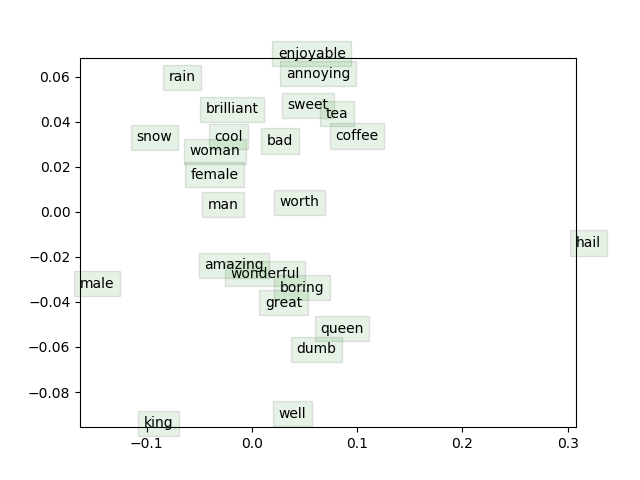
\includegraphics[width=0.6\textwidth]{word_vectors.png}
    \caption{Visualization for the word vectors obtained after training.}
    \label{fig:word2vec}
\end{figure}
    
\begin{shaded}
\begin{answer}

\end{answer}
\end{shaded}

\section{Submission Instructions}
You shall submit this assignment on Gradescope as two submissions -- one for ``Assignment 2 [coding]" and another for `Assignment 2 [written]":
\begin{enumerate}
    \item Run the \texttt{collect\_submission.sh} script to produce your \texttt{assignment2.zip} file.
    \item Upload your \texttt{assignment2.zip} file to Gradescope to ``Assignment 2 [coding]".
    \item Upload your written solutions to Gradescope to ``Assignment 2 [written]".
\end{enumerate}

\end{enumerate}
\end{document}
